\documentclass[a4paper,11pt]{article}
\usepackage[a4paper,vmargin={20mm,20mm},hmargin={30mm,25mm}]{geometry}

\usepackage{graphicx}
\usepackage[utf8]{inputenc}
\usepackage[english,ngerman]{babel}
\usepackage{listings}
\usepackage{xcolor}
\usepackage{verbatim}
%\usepackage{color}
\usepackage{amssymb,amsmath}

\usepackage{caption}
\usepackage{subcaption}

\usepackage{todonotes}
\usepackage{wasysym}

% this makes < > work
\usepackage[T1]{fontenc}

% styles: numeric, alpha
\usepackage[backend=biber,citestyle=alphabetic,bibstyle=alphabetic,url=false,doi=false,isbn=false,maxcitenames=1]{biblatex}
\usepackage[autostyle]{csquotes}
\usepackage{ellipsis}

%\PrerenderUnicode{ü}

\usepackage[pdftex,
            bookmarks,
            pdfauthor={Sebastian Kürten},
            pdftitle={Notes},
            pdfsubject={Notes},
            pdfcreator={pdflatex}]{hyperref}

\hypersetup{
	%linkcolor=[rgb]{0 0 0.5},
	linkcolor=[rgb]{0.1 0.1 0.1},
        colorlinks=true,
        %linktocpage=true,
        linkbordercolor=blue,
        citecolor=[rgb]{0.1 0.1 0.1},
	urlcolor=blue,
        menucolor=red
}

\parindent 0pt                                                                                 
%\parskip 12pt

\widowpenalty=10000

\makeatletter
\renewcommand\paragraph{\@startsection{paragraph}{4}{\z@}%
                                     {-0.5\baselineskip}%
                                     {0.2\baselineskip}%
                                     {\normalfont\normalsize\bfseries}}
\makeatother

\bibliography{literature}
\begin{document}

\selectlanguage{english}

\lstset{
basicstyle=\footnotesize
}

% todolist markers
\newcommand{\itye}{\CheckedBox}
\newcommand{\itno}{\Square}

%%% CONTENT

\title{Images exported via LiveCG}
\author{Sebastian Kürten}
\maketitle

%\tableofcontents

%%% REAL CONTENT

\section{Images}

This document shows some images exported with LiveCG.

\begin{figure}[ht]
	\centering
	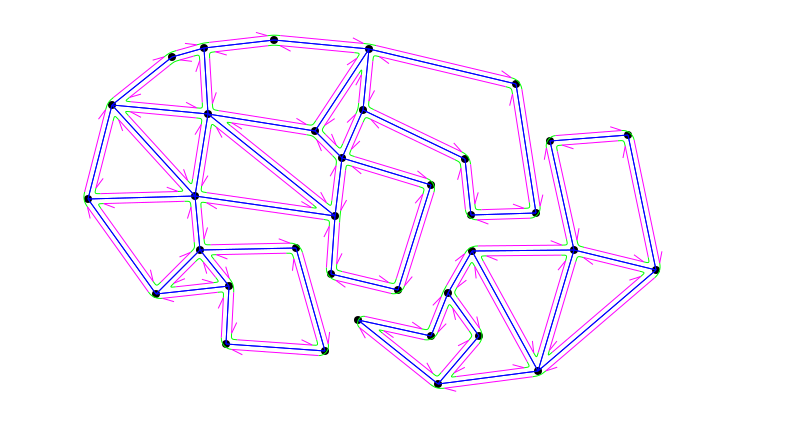
\includegraphics[width=0.8\textwidth]{dcel1.pdf}
	\caption{An arrangement}
	\label{figArrangement1}
\end{figure}

\begin{figure}[ht]
	\centering
	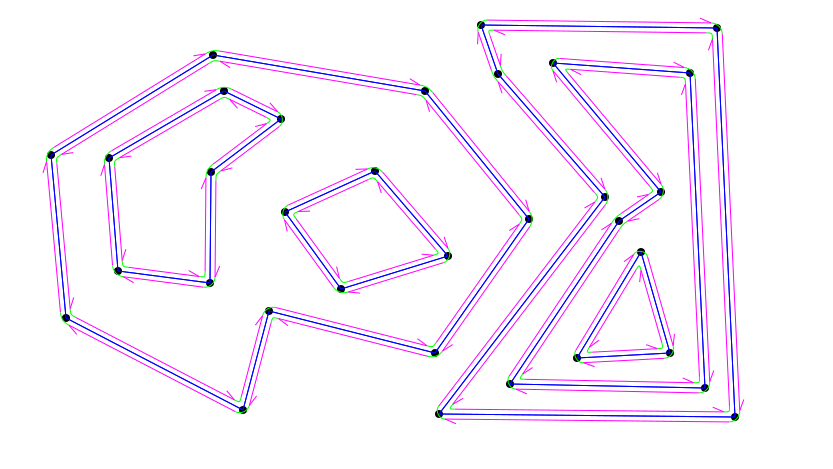
\includegraphics[width=0.8\textwidth]{dcel2.pdf}
	\caption{Another arrangement}
	\label{figArrangement2}
\end{figure}

\begin{figure}[ht]
	\centering
	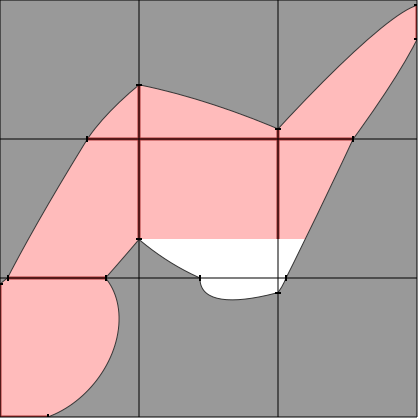
\includegraphics[width=0.8\textwidth]{freespace1.pdf}
	\caption{Free Space diagram}
	\label{figFreeSpace1}
\end{figure}

\begin{figure}[ht]
	\centering
	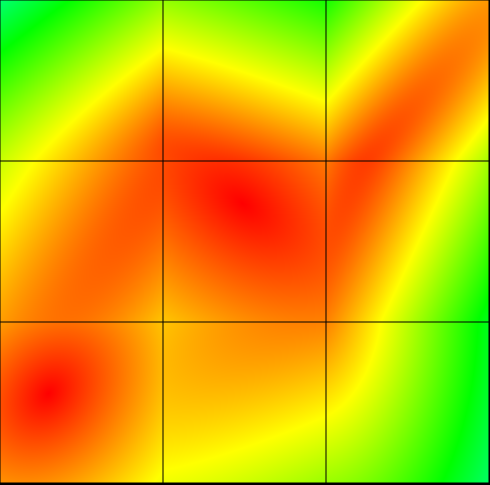
\includegraphics[width=0.8\textwidth]{terrain1.pdf}
	\caption{Distance Terrain}
	\label{figDistanceTerrain1}
\end{figure}

\begin{figure}[ht]
	\centering
	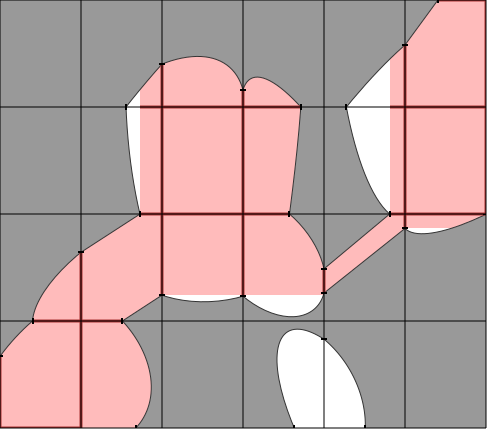
\includegraphics[width=0.8\textwidth]{freespace2.pdf}
	\caption{Free Space diagram}
	\label{figFreeSpace2}
\end{figure}

\begin{figure}[ht]
	\centering
	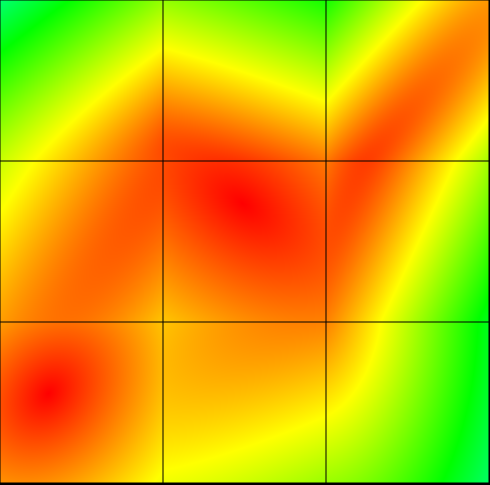
\includegraphics[width=0.8\textwidth]{terrain1.pdf}
	\caption{Distance Terrain}
	\label{figDistanceTerrain2}
\end{figure}

\begin{figure}[ht]
	\centering
	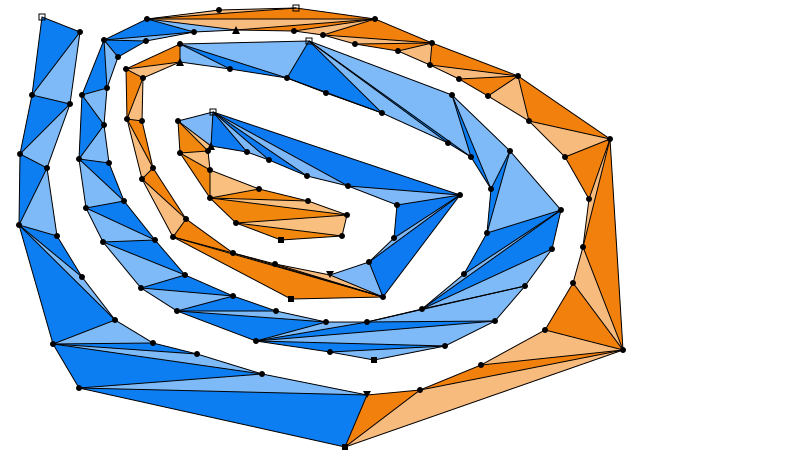
\includegraphics[width=1.0\textwidth]{triangulation.pdf}
	\caption{Polygon triangulation}
	\label{figPolygonTriangulation}
\end{figure}

\begin{figure}[ht]
	\centering
	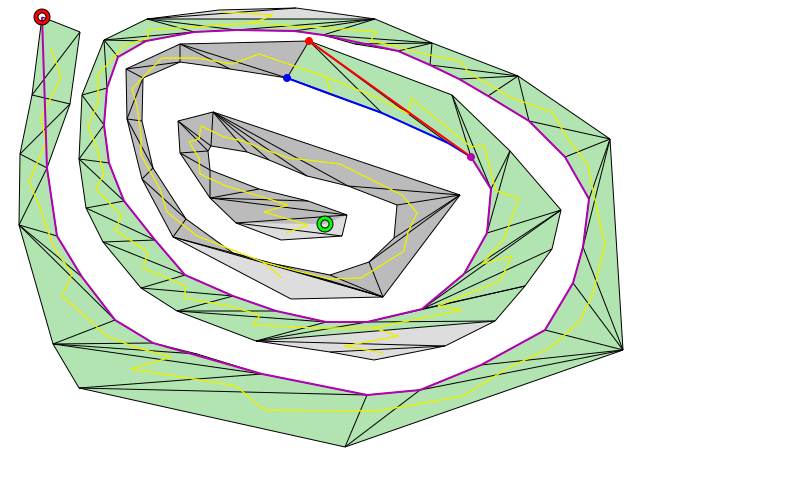
\includegraphics[width=1.0\textwidth]{spip.pdf}
	\caption{Shortest Paths in polygons}
	\label{figSPIP}
\end{figure}

\begin{figure}[ht]
	\centering
	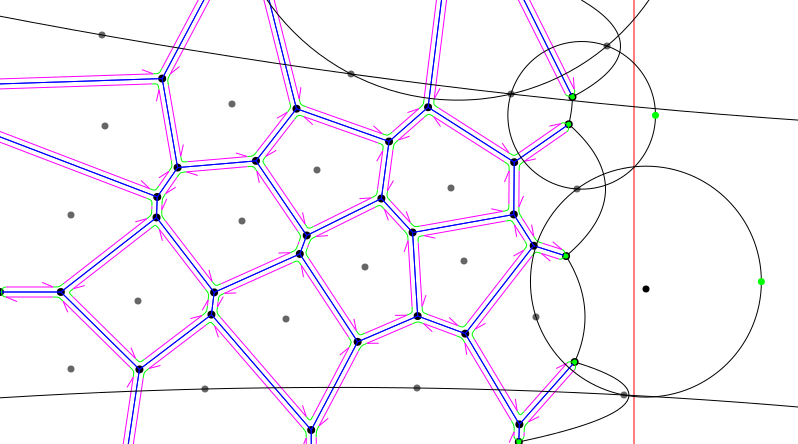
\includegraphics[width=1.0\textwidth]{vorodcel.pdf}
	\caption{Voronoi Diagram with DCEL}
	\label{figVoroDcel}
\end{figure}

\end{document}
